
\documentclass[border=10pt, 12pt]{standalone}
\usepackage[svgnames]{xcolor}
\usepackage{amsmath}
\usepackage{pgfplots}
\pgfplotsset{compat=newest}
\usepackage[sfdefault]{FiraSans}
\usepackage{FiraMono}
\renewcommand*\familydefault{\sfdefault}
\begin{document}
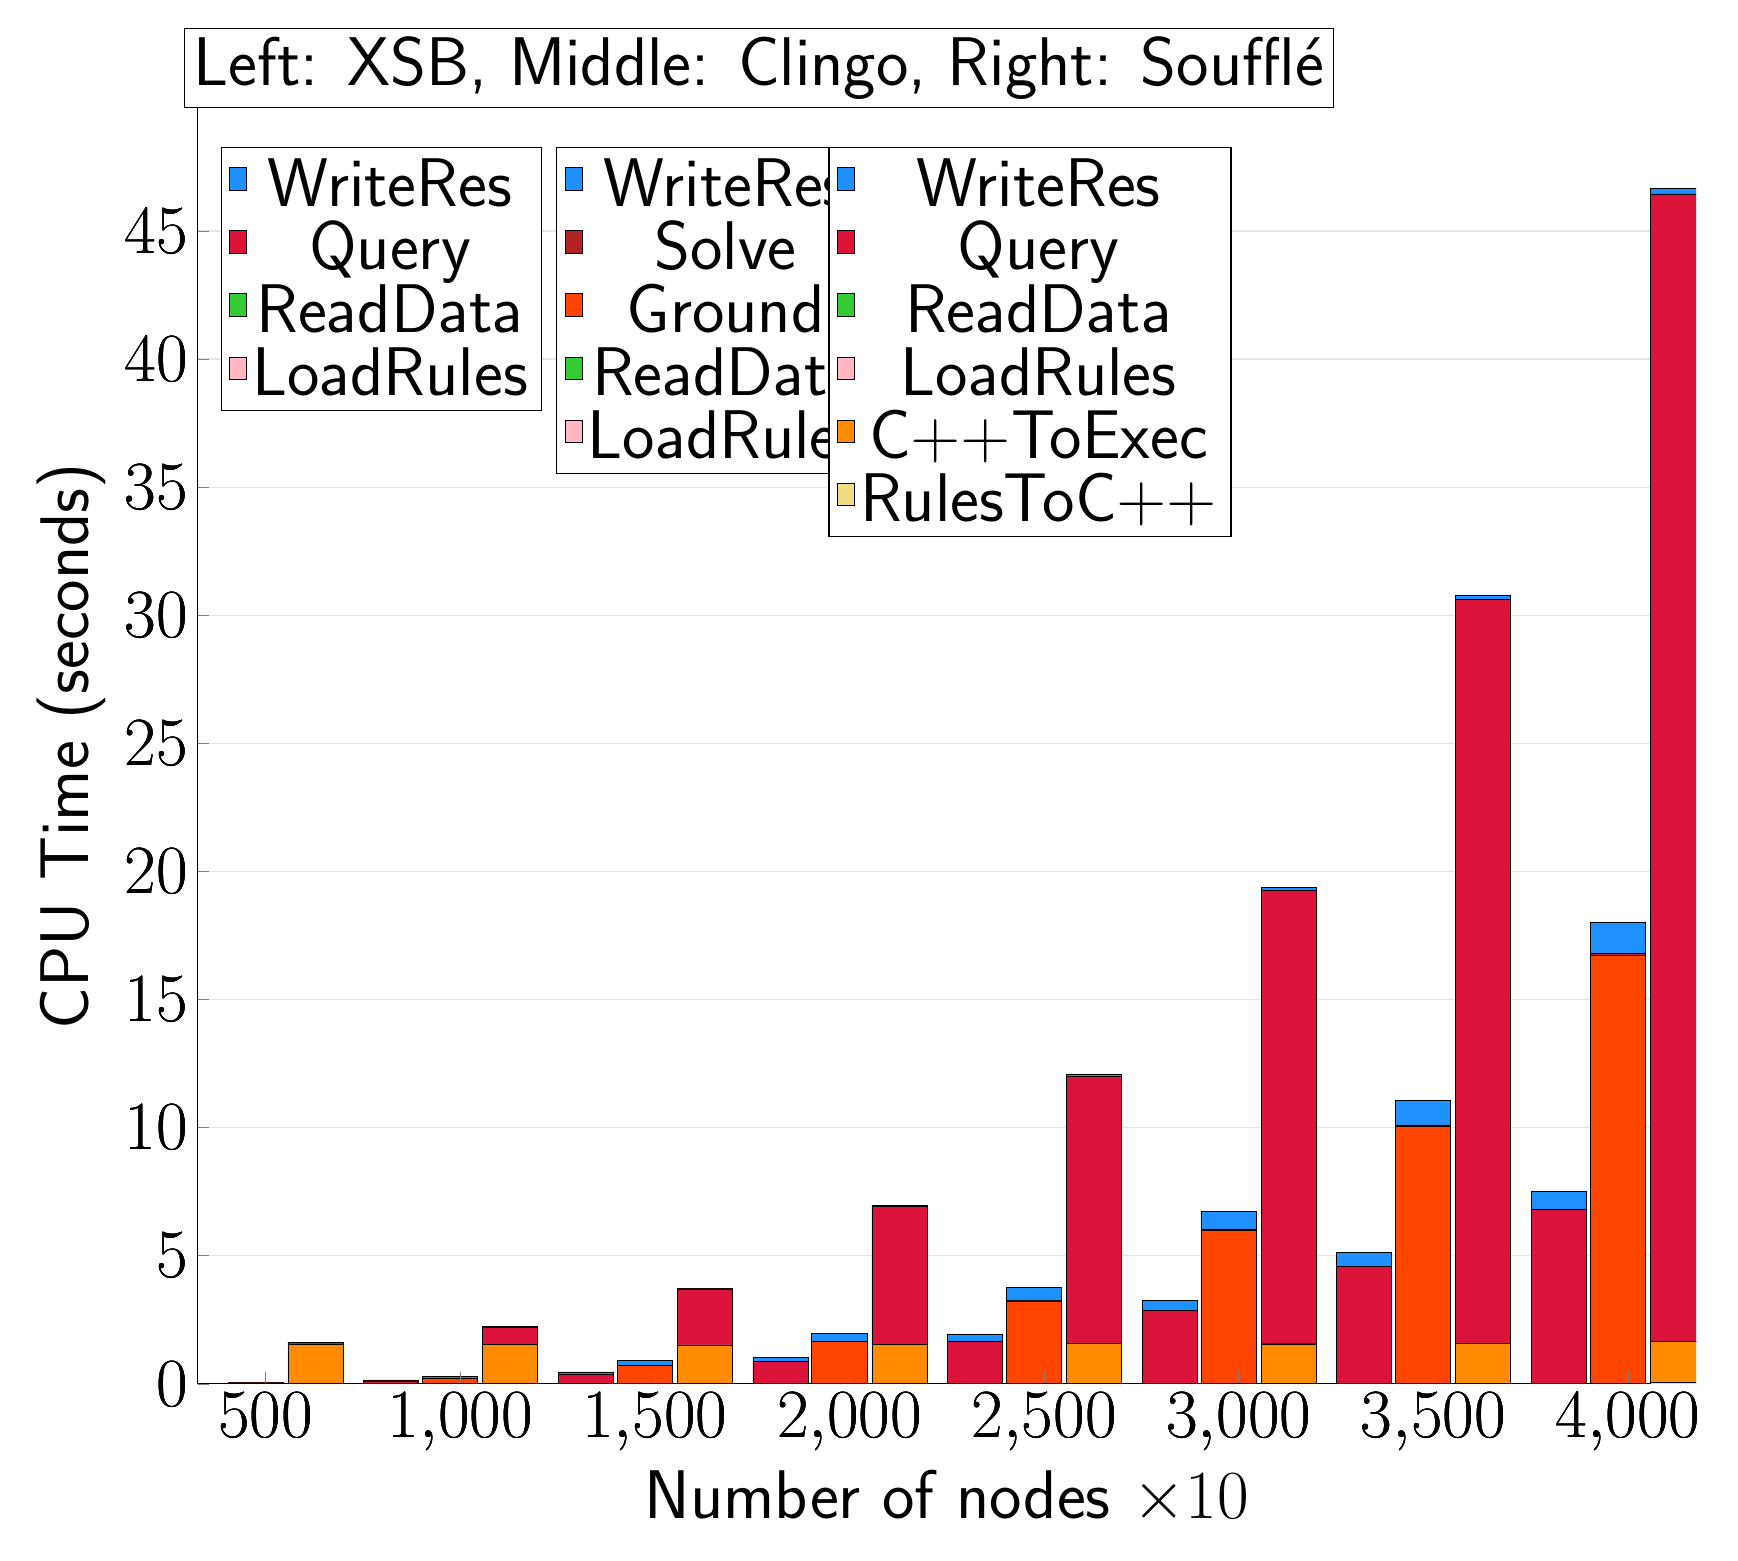
\begin{tikzpicture}
	\begin{axis}[bar shift=-25pt,
			ybar stacked,
			width=1.7\textwidth,
			bar width=0.7cm,
			ymajorgrids, tick align=inside,
			major grid style={draw=gray!20},
			xtick=data,
			ymin=0, ymax=49.78293,
			axis x line*=bottom,
			axis y line*=left,
			enlarge x limits=0.05,
			legend style={
					at={(0.23, 0.97)},
					anchor=north east,
					legend columns=1,
					font=\Huge,
				},
			ylabel={CPU Time (seconds)},
			xlabel={Number of nodes $\times 10$},
			label style={font=\Huge},
			tick label style={font=\Huge},
		]
		\addlegendimage{fill=DodgerBlue, draw=black, line width=0.2pt}
		\addlegendentry{WriteRes}
		\addlegendimage{fill=Crimson, draw=black, line width=0.2pt}
		\addlegendentry{Query}
		\addlegendimage{fill=LimeGreen, draw=black, line width=0.2pt}
		\addlegendentry{ReadData}
		\addlegendimage{fill=LightPink, draw=black, line width=0.2pt}
		\addlegendentry{LoadRules}
		\addplot +[fill=LightPink, draw=black, line width=0.2pt] coordinates {
				(500, 0.0006186000000000002)
				(1000, 0.0006103)
				(1500, 0.0006009000000000003)
				(2000, 0.0006256999999999999)
				(2500, 0.0006299000000000001)
				(3000, 0.0006182999999999998)
				(3500, 0.0006496999999999998)
				(4000, 0.0006337000000000003)
			};
		\addplot +[fill=LimeGreen, draw=black, line width=0.2pt] coordinates {
				(500, 0.0005550999999999996)
				(1000, 0.0010019)
				(1500, 0.0014396)
				(2000, 0.0019598000000000003)
				(2500, 0.0024005000000000003)
				(3000, 0.0028473000000000005)
				(3500, 0.0033237)
				(4000, 0.0037085)
			};
		\addplot +[fill=Crimson, draw=black, line width=0.2pt] coordinates {
				(500, 0.014000199999999999)
				(1000, 0.1090539)
				(1500, 0.3579511000000001)
				(2000, 0.8624541000000001)
				(2500, 1.6583755999999998)
				(3000, 2.8507938)
				(3500, 4.575917)
				(4000, 6.790781300000001)
			};
		\addplot +[fill=DodgerBlue, draw=black, line width=0.2pt] coordinates {
				(500, 0.011263200000000001)
				(1000, 0.0447244)
				(1500, 0.10171960000000002)
				(2000, 0.1764765)
				(2500, 0.28683500000000006)
				(3000, 0.40619570000000016)
				(3500, 0.5543880999999999)
				(4000, 0.7079360999999997)
			};
	\end{axis}

	\begin{axis}[bar shift=-3.7pt,
			ybar stacked,
			width=1.7\textwidth,
			bar width=0.7cm,
			ymajorgrids, tick align=inside,
			major grid style={draw=none},
			xtick=data,
			ymin=0, ymax=49.78293,
			axis x line*=none,
			axis y line*=none,
			enlarge x limits=0.05,
			legend style={
					at={(0.454, 0.97)},
					anchor=north east,
					legend columns=1,
					font=\Huge,
				},
			label style={font=\Huge},
			tick label style={font=\Huge},
		]
		\addlegendimage{fill=DodgerBlue, draw=black, line width=0.2pt}
		\addlegendentry{WriteRes}
		\addlegendimage{fill=FireBrick, draw=black, line width=0.2pt}
		\addlegendentry{Solve}
		\addlegendimage{fill=OrangeRed, draw=black, line width=0.2pt}
		\addlegendentry{Ground}
		\addlegendimage{fill=LimeGreen, draw=black, line width=0.2pt}
		\addlegendentry{ReadData}
		\addlegendimage{fill=LightPink, draw=black, line width=0.2pt}
		\addlegendentry{LoadRules}
		\addplot +[fill=LightPink, draw=black, line width=0.2pt] coordinates {
				(500, 0.0)
				(1000, 0.0)
				(1500, 0.0)
				(2000, 0.0)
				(2500, 0.0)
				(3000, 0.0)
				(3500, 0.0)
				(4000, 0.0)
			};
		\addplot +[fill=LimeGreen, draw=black, line width=0.2pt] coordinates {
				(500, 0.0)
				(1000, 0.0)
				(1500, 0.003999999999999999)
				(2000, 0.009999999999999997)
				(2500, 0.009999999999999997)
				(3000, 0.008999999999999998)
				(3500, 0.009999999999999997)
				(4000, 0.009999999999999997)
			};
		\addplot +[fill=OrangeRed, draw=black, line width=0.2pt] coordinates {
				(500, 0.03799999999999999)
				(1000, 0.22400000000000003)
				(1500, 0.715)
				(2000, 1.6420000000000001)
				(2500, 3.2239999999999993)
				(3000, 5.990999999999999)
				(3500, 10.032)
				(4000, 16.701)
			};
		\addplot +[fill=FireBrick, draw=black, line width=0.2pt] coordinates {
				(500, 0.001999999999999999)
				(1000, 0.0050000000000000044)
				(1500, 0.01200000000000001)
				(2000, 0.017999999999999995)
				(2500, 0.031000000000000007)
				(3000, 0.04400000000000008)
				(3500, 0.062000000000000145)
				(4000, 0.07699999999999949)
			};
		\addplot +[fill=DodgerBlue, draw=black, line width=0.2pt] coordinates {
				(500, 0.018000000000000006)
				(1000, 0.07400000000000002)
				(1500, 0.181)
				(2000, 0.31100000000000005)
				(2500, 0.48999999999999994)
				(3000, 0.7009999999999998)
				(3500, 0.9649999999999996)
				(4000, 1.2430000000000003)
			};
	\end{axis}

	\begin{axis}[bar shift=18pt,
			ybar stacked,
			width=1.7\textwidth,
			bar width=0.7cm,
			ymajorgrids, tick align=inside,
			major grid style={draw=none},
			xtick=data,
			ymin=0, ymax=49.78293,
			axis x line*=none,
			axis y line*=none,
			enlarge x limits=0.05,
			legend style={
					at={(0.69, 0.97)},
					anchor=north east,
					legend columns=1,
					font=\Huge,
				},
			label style={font=\Huge},
			tick label style={font=\Huge},
		]
		\addlegendimage{fill=DodgerBlue, draw=black, line width=0.2pt}
		\addlegendentry{WriteRes}
		\addlegendimage{fill=Crimson, draw=black, line width=0.2pt}
		\addlegendentry{Query}
		\addlegendimage{fill=LimeGreen, draw=black, line width=0.2pt}
		\addlegendentry{ReadData}
		\addlegendimage{fill=LightPink, draw=black, line width=0.2pt}
		\addlegendentry{LoadRules}
		\addlegendimage{fill=DarkOrange, draw=black, line width=0.2pt}
		\addlegendentry{C++ToExec}
		\addlegendimage{fill=LightGoldenrod, draw=black, line width=0.2pt}
		\addlegendentry{RulesToC++}
		\addplot +[fill=LightGoldenrod, draw=black, line width=0.2pt] coordinates {
				(500, 0.030000000000000006)
				(1000, 0.030000000000000006)
				(1500, 0.030000000000000006)
				(2000, 0.030000000000000006)
				(2500, 0.032999999999999995)
				(3000, 0.034999999999999996)
				(3500, 0.03799999999999999)
				(4000, 0.043)
			};
		\addplot +[fill=DarkOrange, draw=black, line width=0.2pt] coordinates {
				(500, 1.496)
				(1000, 1.5050000000000003)
				(1500, 1.4820000000000002)
				(2000, 1.506)
				(2500, 1.5349999999999997)
				(3000, 1.5240000000000002)
				(3500, 1.544)
				(4000, 1.6099999999999999)
			};
		\addplot +[fill=LightPink, draw=black, line width=0.2pt] coordinates {
				(500, 9.44e-05)
				(1000, 9.980000000000001e-05)
				(1500, 0.00011889999999999999)
				(2000, 0.00010740000000000001)
				(2500, 0.00011359999999999998)
				(3000, 0.0001081)
				(3500, 8.7e-05)
				(4000, 0.0001343)
			};
		\addplot +[fill=LimeGreen, draw=black, line width=0.2pt] coordinates {
				(500, 0.0011719999999999999)
				(1000, 0.0021666000000000003)
				(1500, 0.003399)
				(2000, 0.0042295)
				(2500, 0.0047832)
				(3000, 0.005888299999999999)
				(3500, 0.006410400000000001)
				(4000, 0.0084299)
			};
		\addplot +[fill=Crimson, draw=black, line width=0.2pt] coordinates {
				(500, 0.09771330000000002)
				(1000, 0.6800317)
				(1500, 2.187298)
				(2000, 5.37517)
				(2500, 10.44145)
				(3000, 17.694200000000002)
				(3500, 29.03066)
				(4000, 44.78293)
			};
		\addplot +[fill=DodgerBlue, draw=black, line width=0.2pt] coordinates {
				(500, 0.0036627)
				(1000, 0.014149799999999999)
				(1500, 0.0316058)
				(2000, 0.055704699999999996)
				(2500, 0.0871951)
				(3000, 0.12498519999999999)
				(3500, 0.17109460000000004)
				(4000, 0.22383570000000003)
			};
	\end{axis}


	\node[anchor=south, draw, fill=white] at (rel axis cs:0.42,1) {\Huge Left: XSB, Middle: Clingo, Right: Soufflé};
\end{tikzpicture}
\end{document}
